\documentclass[10pt,a4paper]{article}
\usepackage[utf8]{inputenc}
\usepackage[T1]{fontenc}
\usepackage{lmodern}
\usepackage[margin=1.5cm, top=1.4cm, bottom=1.4cm]{geometry}
\usepackage{hyperref}
\usepackage{enumitem}
\usepackage{titlesec}
\usepackage{xcolor}
\usepackage{graphicx}

\definecolor{accent}{HTML}{00686E}
\hypersetup{colorlinks=true, urlcolor=accent, linkcolor=accent}
\pagenumbering{arabic}
\setlength{\parindent}{0pt}

\titleformat{\section}{\large\bfseries\color{accent}}{}{0em}{}[\vspace{-0.6em}\rule{\textwidth}{0.8pt}]
\titlespacing{\section}{0pt}{7pt}{4pt}

\newcommand{\role}[4]{%
  \textbf{#1} \hfill \textbf{#2}\\[1pt]%
  \textit{#3} \hfill \textit{#4}\\[2pt]%
}
\setlist[itemize]{leftmargin=1.2em, itemsep=1.5pt, topsep=2pt, parsep=0pt}

\begin{document}

% ================= HEADER =================
\begin{minipage}[c]{0.80\textwidth}
  {\Huge\bfseries Prabhavit Gupta}\\[3pt]
  {\color{accent}\large Senior AI Solutions Engineer: GTM Automation, AI Agents \& Enterprise Integrations}\\[6pt]
  {\footnotesize +39 351 610 7807 ~$\vert$~
  \href{mailto:prabhavitg@gmail.com}{prabhavitg@gmail.com} ~$\vert$~
  \href{https://www.linkedin.com/in/prabhavit/}{linkedin.com/in/prabhavit} ~$\vert$~
  \href{https://github.com/prab-gupta}{github.com/prab-gupta} ~$\vert$~
  Venice, Italy}
\end{minipage}\hfill
\begin{minipage}[c]{0.18\textwidth}
  \raggedleft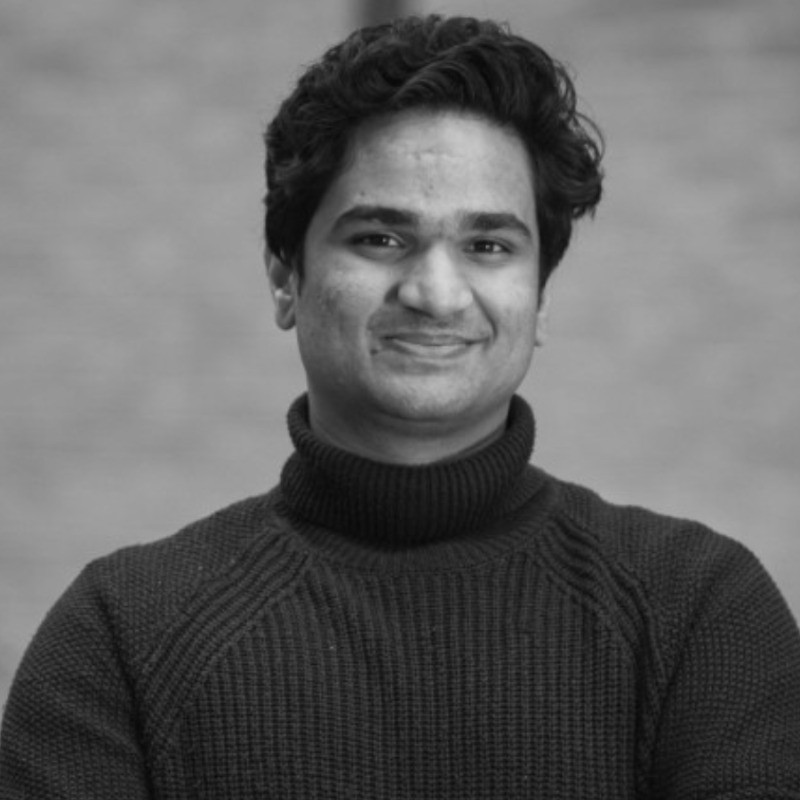
\includegraphics[width=2.0cm]{photo.jpg}
\end{minipage}
\vspace{-2pt}

% ================= SUMMARY =================
\section{Summary}
AI Solutions and Integration Engineer with 3 years of hands-on experience designing, shipping, and evaluating production LLM agents, GTM automations, and scalable workflow integrations across European tech environments. At FlowSpace, architected multi-step sales automation and lead enrichment pipelines, built automated document ingestion systems extracting structured data across 900+ records, deployed autonomous customer support agents with live API tool use and fallback routing, and directed developer workflows with Claude Code, TypeScript, and working-level Python. Experienced with CRM synchronization, idempotent webhook reconciliation, RESTful API architecture, and prompt engineering across Anthropic, OpenAI, and Google models. Based in Venice, Italy with an EU Long Term Residence Permit (unrestricted EU work authorization without sponsorship). Immediately available.

% ================= TECHNICAL EXPERTISE =================
\section{Technical Expertise}
\begin{itemize}
  \item \textbf{AI Solutions \& Agentic Systems:} Autonomous agent workflows, Multi-step agent orchestration, Tool calling, Function calling, Prompt engineering, Structured JSON schemas, Context management, Gemini, Claude, OpenAI APIs.
  \item \textbf{GTM \& Automation:} GTM pipelines, Sales funnel automations, Lead enrichment \& capture, CRM integrations, n8n, Playwright, Webhooks, Postman.
  \item \textbf{Full Stack \& Integration Engineering:} TypeScript, JavaScript, Node.js, Working-level Python, Laravel, RESTful APIs, WebSockets, PostgreSQL, Supabase, Docker, Git.
  \item \textbf{Project \& Business Acumen:} Cross-functional collaboration, Translating business challenges into technical specifications, Rapid prototyping, QA verification.
  \item \textbf{Languages \& Work Authorization:} Hindi (Native), English (C1 Professional), Italian (Beginner). EU Long Term Residence Permit (No EU sponsorship required).
\end{itemize}

% ================= EXPERIENCE =================
\section{Experience}

\role{\href{https://flowspace.co}{FlowSpace.co}}{Mar 2024 - Aug 2026}{Lead Developer (Full-time, Freelance)}{London, UK (remote)}
\begin{itemize}
  \item Engineered end-to-end GTM automations for sales funnels, automated lead capture, and lead enrichment across multiple business systems, consolidating CRM records and streamlining revenue operations.
  \item Architected and deployed production customer support AI agents using LLM tool calling and live REST API function calling to query platform availability and execute bookings, with confidence thresholds and fallback routing.
  \item Built an automated knowledge ingestion and listing bot with human-in-the-loop review: parsed heterogeneous documents (PDFs, spreadsheets, web pages) into structured database records using LLM extraction prompts, creating 900+ verified listings.
  \item Engineered agentic developer workflows and tooling using Claude Code, TypeScript, and automated testing, accelerating feature delivery cycles across the engineering team.
  \item Directed platform architecture migration off a legacy stack to a modern Next.js, TypeScript, and Laravel backend, establishing reliable schema contracts and API specifications.
  \item Integrated external REST APIs (OfficeRnD, Nexudus, Stripe) with idempotent event handling and automated webhook reconciliation.
  \item Implemented token tracking, prompt versioning, and end-to-end regression testing with Playwright to maintain high output fidelity across production agent runs.
  \item Scaled platform user base from 2,000 to 4,500+ active users through iterative product engineering and resilient backend automations.
\end{itemize}

\role{Urlink}{Apr 2025 - Jul 2025}{Project Manager \& AI Assisted Developer (Freelance)}{Barcelona, Spain (remote)}
\begin{itemize}
  \item Led technical delivery of AI-assisted web applications, coordinating API contracts, database schemas, and external integrations.
  \item Evaluated commercial LLM APIs (OpenAI, Anthropic) across task types, optimizing prompt structures and model selection for latency and output consistency.
  \item Implemented automated CI/CD checks and test suites, ensuring clean code releases and minimal deployment regressions.
\end{itemize}

\role{Independent Technical Consultant}{Aug 2023 - Feb 2024}{AI Solutions \& Automation Engineer}{Venice, Italy}
\begin{itemize}
  \item Developed custom AI automations, agent prototypes, and data extraction pipelines for European SME clients using n8n, Playwright, and LLM APIs.
  \item Implemented idempotent webhook listeners and CRM data synchronization flows, replacing error-prone manual administrative processes.
  \item Built prototype RAG inquiry assistants integrated with company documentation for rapid customer response triage.
\end{itemize}

% ================= EDUCATION =================
\section{Education}
\role{Ca' Foscari University of Venice}{2020 - 2024}{BA in Philosophy, International Studies and Economics}{Venice, Italy}
\begin{itemize}
  \item In-depth focus on formal logic, analytical problem solving, systems analysis, and macroeconomic decision models.
\end{itemize}

\end{document}
